\documentclass{article}
\usepackage{tikz}

% Delete page number
\pagenumbering{gobble}

\usetikzlibrary{trees, positioning, calc}


\begin{document}

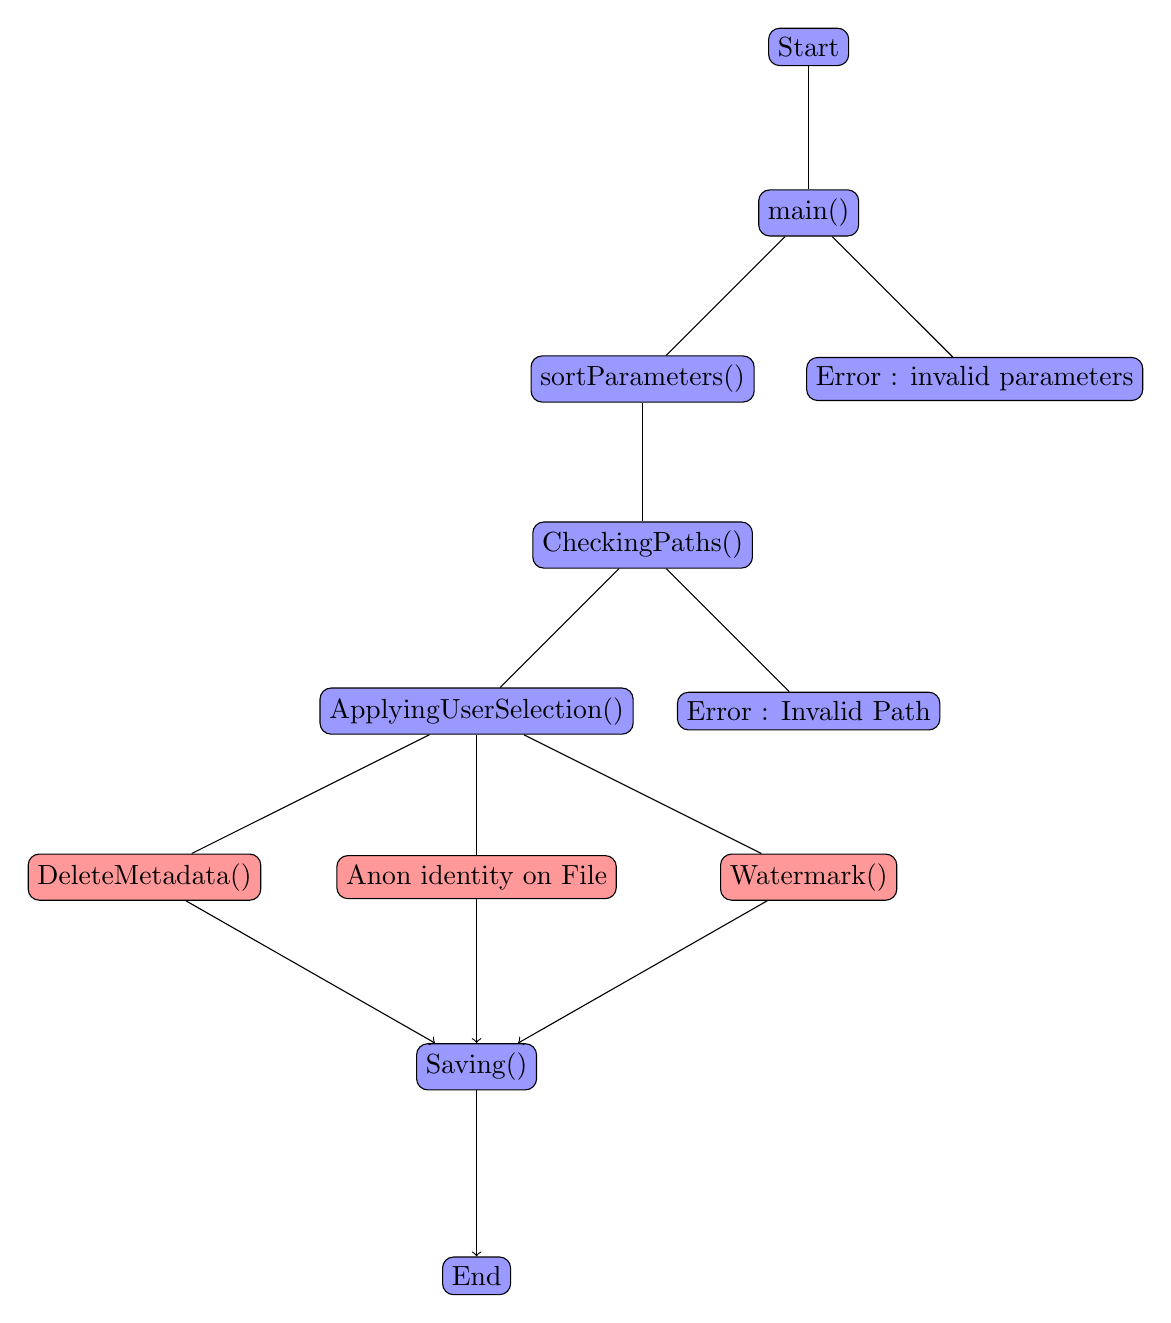
\begin{tikzpicture}[
    sibling distance=12em,
    level distance=6em,
    every node/.style={rectangle, rounded corners, draw, align=center, top color=blue!40, bottom color=blue!40},
    special/.style={rectangle, rounded corners, draw, align=center, top color=red!40, bottom color=red!40}
]

\node {Start}
  child { node {main()}
    child {node {sortParameters()}
      child {node {CheckingPaths()}
        child {node {ApplyingUserSelection()}
          child {node (delete) [special] {DeleteMetadata()}}
          child {node (anon) [special] {Anon identity on File}}
          child {node (water) [special] {Watermark()}}
        }
        child {node {Error : Invalid Path}}
      }
    }
    child {node {Error : invalid parameters}}
  };

% Merged node
\node (merged) [below=6em of $(delete)!0.5!(water)$, rectangle, draw, rounded corners, top color=blue!40, bottom color=blue!40, align=center] {Saving()};

% Connect last three children to merged node
\draw[->] (delete) -- (merged);
\draw[->] (anon) -- (merged);
\draw[->] (water) -- (merged);

% Continue after merged
\node (final) [below=6em of merged, rectangle, draw, rounded corners, top color=blue!40, bottom color=blue!40, align=center] {End};

\draw[->] (merged) -- (final);

\end{tikzpicture}

\end{document}
